\documentclass{article}

\usepackage{polski}
\usepackage[utf8]{inputenc}
\usepackage{graphicx}
\usepackage{float}
\usepackage{textcomp}

\begin{document}
	
	\pagenumbering{gobble}
		\begin{titlepage}
		\centering
		
		 \Huge{
		 	\indexspace Projekt zespołowy \\ 
		 	\indexspace Aplikacja internetowa do zarządzania finansami \\[1cm]
		 	\indexspace \textbf{"Where's my money?!"\\[1cm]}}
		
		
\includegraphics[width=5cm]{assets/logo.png}\\[1cm]
		\Large{Patryk Mroczyński \\ \textlangle{}\textit{patryk.mroczynski@student.put.poznan.pl}\textrangle{} \\126810\\
		Oskar Rutkowski \\ \textlangle{}\textit{oskar.rutkowski@student.put.poznan.pl}\textrangle{} \\126845 \\
		Jakub Wiśniewski \\ \textlangle{}\textit{jakub.t.wisniewski@student.put.poznan.pl}\textrangle{} \\126824 \\[0.5cm]}
	\today
		
	\end{titlepage}
	\newpage
	\tableofcontents
	\newpage
	\pagenumbering{arabic}

	\section{Charakterystyka ogólna projektu}
	\paragraph{} Aplikacja ma na celu uproszczenie zarządzania budżetem domowym użytkownika. Umożliwia ona dodawanie wydatków i przychodów wraz z przypisaniem im odpowiednich kategorii. Dodawanie może odbywać się albo jako importowanie pliku w formacie CSV, który jest generowany przez użytkownika na stronie banku, albo poprzez ręczne wpisanie przez użytkownika kwoty i przydzielenia kategorii. Użytkownik może definiować subkonta, do których przypisywane są wydatki. Aplikacja umożliwia generowanie raportów i wykresów dla określonego przedziału czasowego z uwzględnieniem tylko wybranych kategorii czy subkont, które są wybrane przez użytkownika. Użytkownik ma możliwość eksportowania raportów do wybranego formatu.
	\section{Architektura systemu}
	\paragraph{} System oparty jest na modelu klient-serwer, gdzie klient (łącznie z interfejsem i logiką po stronie klienta) jest uruchamiany w przeglądarce, a na maszynie serwerowej działa relacyjna baza danych oraz program, który wykonuje operacje na bazie danych i udostępnia API, z którego korzysta aplikacja kliencka. Serwer składa się z mikrousług, które udostępniają metody zgodnie z architekturą REST. \\[0.5cm]
	Serwer składa się z mikroserwisów, które udostępniają odpowiednie metody protokołu HTTP dla klienta.
	
	\subsection{Mikroserwisy}
	W podrozdziale zostały wylistowane mikroserwisy, z których składa się serwer wraz z ich 
	metodami.
	\begin{itemize}
		\item AuthApi - służy do autoryzacji użytkowników.
		\item UserApi
			\begin{itemize}
				\item \textbf{GET /api/users/} - zwraca listę użytkowników z bazy danych.
				
				\item \textbf{GET /api/users/:id/} - zwraca szczegóły użytkownika o podanym id.
				
				\item \textbf{POST /api/users/} - tworzy nowego użytkownika.
				
				\item \textbf{PUT /api/users/:id} - aktualizuje informacje o użytkowniku.
				
				\item \textbf{DELETE /api/users/:id/} - usuwa użytkownika o podanym id.
				
			\end{itemize}
		\item SubaccountApi
			\begin{itemize}
				\item \textbf{GET /api/subaccounts/:id} - zwraca listę subkont dla użytkownika.
				
				\item \textbf{POST /api/subaccounts/} - dodaje nowe subkonto.
				
				\item \textbf{PUT /api/subaccounts/:id/} - aktualizuje informacje o subkoncie o danym id.
				
				\item \textbf{DELETE /api/subaccounts/:id/} - usuwa subkonto o podanym id.
			\end{itemize}
		\item TransactionApi
			\begin{itemize}
				\item \textbf{GET /api/transactions/} - zwraca listę transakcji dla użytkownika.
				
				\item \textbf{GET /api/transactions/:id/} - zwraca szczegóły transakcji o podanym id.
				
				\item \textbf{POST /api/transactions/} - dodaje nową transakcję do historii.
				
				\item \textbf{PUT /api/transactions/:id/} - aktualizuje informacje o transakcji.
				
				\item \textbf{DELETE /api/transactions/:id/} - usuwa transakcję o podanym id.
			\end{itemize}
		\item CsvSettingApi
			\begin{itemize}
				\item \textbf{GET /api/csvsettings/} - zwraca listę predefiniowanych ustawień arkuszy dla banków oraz własne ustawienia użytkownika.
				
				\item \textbf{GET /api/csvsettings/:id/} - zwraca pojedyncze ustawienie CSV.
				
				\item \textbf{POST /api/csvsettings/} - tworzy nowe ustawienie arkusza.
				
				\item \textbf{PUT /api/csvsettings/:id/} - aktualizuje informacje o ustawieniu arkusza.
				
				\item \textbf{DELETE /api/csvsettings/:id/} - usuwa ustawienie arkusza o podanym id.
			\end{itemize}
		\item CategoryApi
			\begin{itemize}
				\item \textbf{GET /api/categories/} - zwraca listę predefiniowanych kategorii oraz własnych użytkownika.
				
				\item \textbf{POST /api/categories/} - dodaje nową kategorię.
				
				\item \textbf{PUT /api/categories/:id/} - aktualizuje informacje o kategorii.
				
				\item \textbf{DELETE /api/categories/:id/} - usuwa kategorię o podanym id.
			\end{itemize}
		\item CategoryMappingApi
			\begin{itemize}
				\item \textbf{GET /api/categorymapping/} - zwraca listę mapowań dla użytkownika.
				
				\item \textbf{POST /api/categorymapping/} - dodaje nowe mapowanie.
				
				\item \textbf{PUT /api/categorymapping/:id/} - aktualizuje informacje o mapowaniu o danym id.
				
				\item \textbf{DELETE /api/categorymapping/:id/} - usuwa mapowanie o podanym id.
			\end{itemize}
	\end{itemize}
	\section{Wymagania}
	\paragraph{} W rozdziale opisane są wymagania funkcjonalne oraz niefunkcjonalne z podziałem na aktorów.
	\subsection{Wymagania funkcjonalne}
	W wymaganiach funkcjonalnych wyszczególnionych jest dwóch aktorów: użytkownik niezalogowany oraz użytkownik zalogowany.
	\begin{itemize}
		\item Niezalogowany użytkownik może skorzystać z wersji testowej aplikacji bez rejestracji.
		\item Niezalogowany użytkownik może się zarejestrować oraz zalogować.
		\item Niezalogowany użytkownik ma możliwość wysłania prośby o zresetowanie hasła poprzez podanie adresu email.
		\item Zalogowany użytkownik może się wylogować
		\item Zalogowany użytkownik może w opcjach konta edytować adres email, hasło oraz nazwę konta.
		\item Zalogowany użytkownik może tworzyć subkonta, do których przypisuje wybrane wydatki oraz przychody.
		\item Zalogowany użytkownik może dodawać wyciąg z konta dowolnego banku jako plik w formacie CSV.
		\item Zalogowany użytkownik może ręcznie dodać wpis, wpisując kwotę oraz dobierając kategorię, a także walutę.
		\item Zalogowany użytkownik ma możliwość modyfikacji i usuwania wpisów w aplikacji.
		\item Zalogowany użytkownik może generować raporty z określonego przedziału czasowego dla określonych kategorii i subkont.
		\item Zalogowany użytkownik może eksportować swoje raporty finansowe jako pliki w formacie CSV lub PDF.
		\item Zalogowany użytkownik przy dodawaniu wyciągu konta może wybrać układ pliku CSV między predefiniowanymi bankami lub zdefiniowanym przez siebie układem.
		\item Zalogowany użytkownik może dodać wzór tytułu oraz dopasować do niego kategorię, aby zautomatyzować uzupełnianie kategorii przy dodawaniu wpisów z pliku w formacie CSV.
		\item Zalogowany użytkownik może dodawać komentarze do wpisów.
		
	\end{itemize}
	\subsection{Wymagania niefunkcjonalne}
	W wymaganiach funkcjonalnych wyszczególnionych jest trzech aktorów: użytkownik, aplikacja serwerowa oraz aplikacja kliencka.
	\begin{itemize}
		\item Aplikacja serwerowa napisana w języku Python3.
		\item Aplikacja serwerowa wykorzystuje relacyjną bazę danych PostgreSQL.
		\item Osobna baza danych dla wersji testowej oraz dla pełnej wersji dla zalogowanych użytkowników.
		\item Aplikacja nie wymaga od użytkownika instalowania dodatkowego oprogramowania poza aktualną przeglądarką.
		\item Wykorzystanie architektury PWA (z ang. Progressive Web Applications) w celu instalowania aplikacji na urządzeniach mobilnych.
		\item Aby użytkownik mógł korzystać z aplikacji musi się poprawanie zalogować na założone w serwisie konto.
		\item Dane użytkownika są przechowywane w bazie danych.
		\item Hasło użytkownika przechowywane jest jako wynik funkcji skrótu SHA-256.
		\item Hasło użytkownika ma minimum 8 znaków długości oraz składa się z co najmniej jednej cyfry, jednego znaku specjalnego, jednej wielkiej litery i jednej małej litery.
		\item System logowania oparty o metodę Basic Auth.
		\item Aplikacja kliencka jest zaprojektowana zgodnie z techniką Responsive Web Design.
		\item API stworzone jest zgodnie z architekturą REST, w formie mikroserwisów.
		\item Raporty mają formę tabeli lub wykresu.
	\end{itemize}
	\section{Narzędzia, środowiska, biblioteki}
	\paragraph{}Serwer działa w oparciu o system operacyjny Ubuntu Server 16.04 LTS.
	Do zarządzania danymi wykorzystywana jest relacyjna baza danych PostgreSQL w wersji 9.6.8.
	Mikroserwisy działające jako aplikacja serwerowa napisane są w języku Python 3.6 wraz z frameworkiem CherryPy 14.0 oraz adapterem Psycopg 2.7.4. 
	\paragraph*{} Aplikacja kliencka to interaktywna strona internetowa, napisana przy pomocy frameworka React dla języka JavaScript, w którym wykorzystywany jest także język HTML5 oraz CSS3 z preprocesorem LESS. Do tworzenia aplikacji jest używany język EcmaScript 2017 w standardzie ECMA-262, który kompilowany jest przy pomocy kompilatora Babel do języka JavaScript. Strona może być poprawnie wyświetlona na dowolnej aktualnej przeglądarce internetowej.
	\paragraph*{} Dodatkowe narzędzia wykorzystane przy tworzeniu aplikacji to Visual Studio Code 1.20.1, DBeaver Community Edition 5.0, Wireshark 2.4.5 
	\paragraph*{} Narzędzia, które zostały wykorzystane do wspierania pracy zespołowej to Trello.com do organizacji zadań, system kontoli wersji Git wraz z repozytorium na stronie GitHub.com, TexStudio (z użyciem MiKTeX) do tworzenia dokumentacji oraz Microsoft Visio do tworzenia schematów oraz diagramów.
	\section{Najważniejsze protokoły}
	\paragraph*{} 
	Użytkownik komunikuje się z serwerem poprzez protokół HTTPS (z ang. Hypertext Transfer Protocol Secure) w warstwie aplikacji, który wykorzystuje TLS (z ang. Transport Layer Security) w wartstwie prezentacji do szyfrowania danych wysyłanych do serwera i odszyfrowywania danych otrzymywanych. TLS wykorzystuje do transportu protokół TCP w warstwie transportowej.
	\section{Schemat bazy danych}
	\paragraph{} W rozdziale opisane zostały relacje pomiędzy tabelami w relacyjnej bazie danych. 
	\begin{figure}[H]
		\centering
		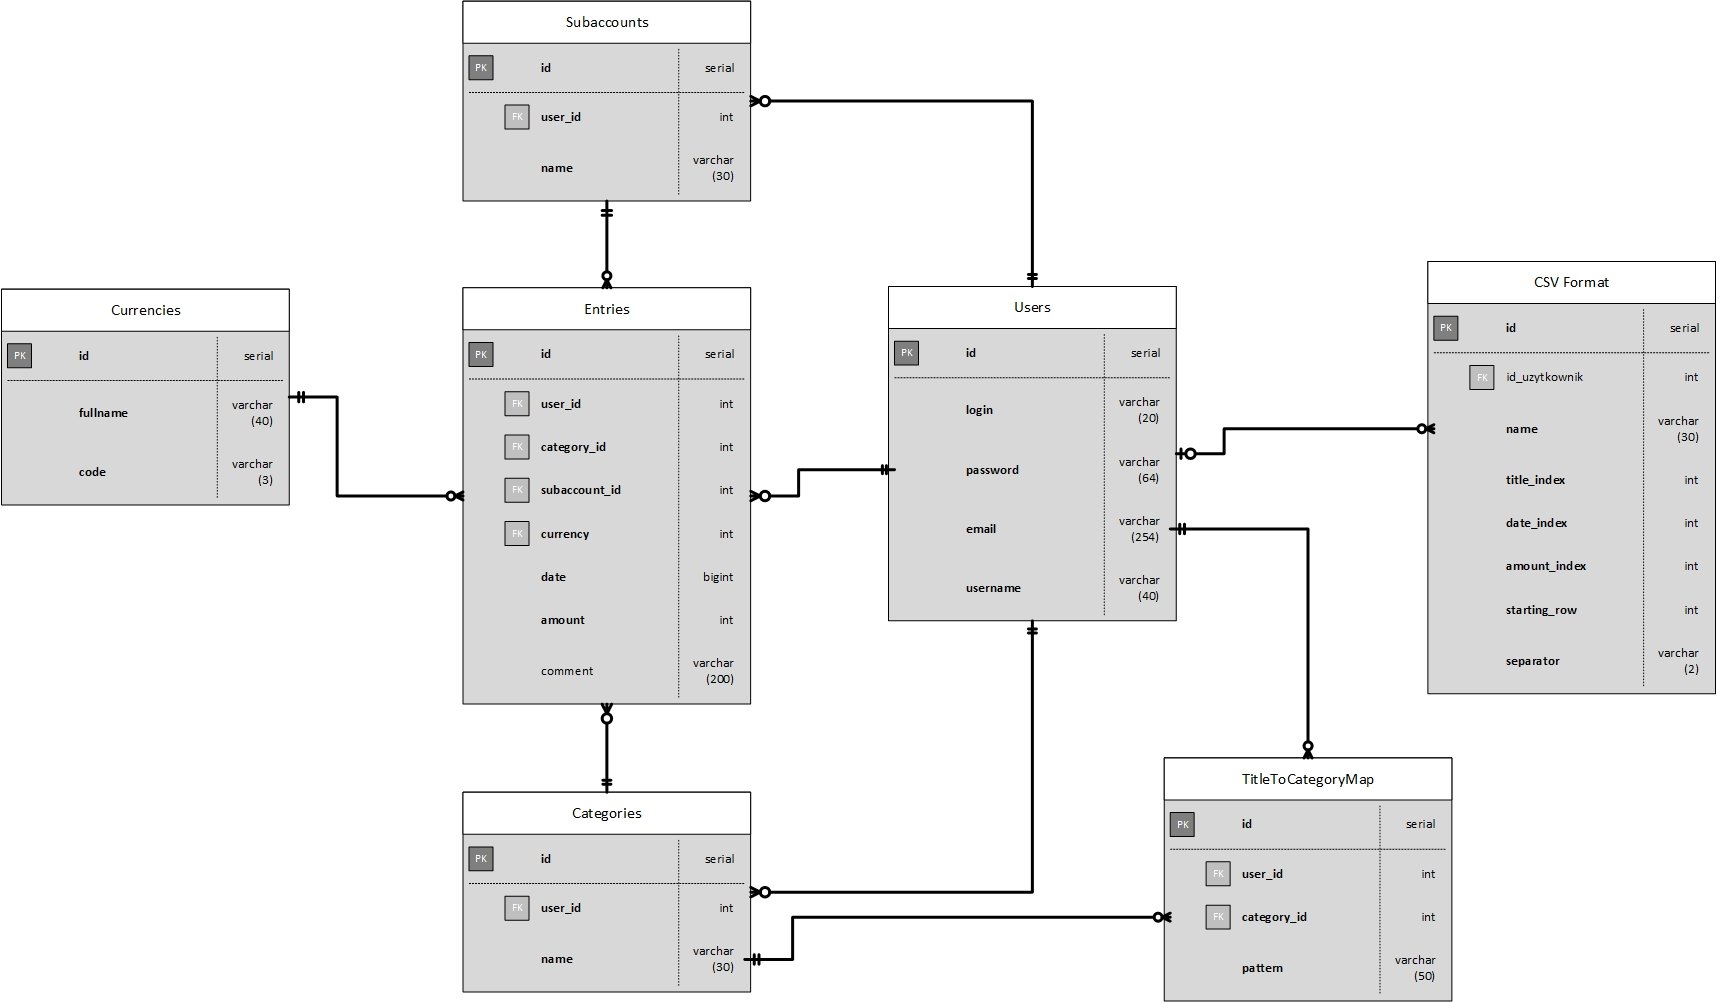
\includegraphics[width=0.8\linewidth]{assets/er.jpg}
		\caption[]{Schemat relacyjny}
		\label{fig:er}
	\end{figure}
	
	Zgodnie z rysunkiem \ref{fig:er}, w bazie danych znajduje się siedem tabel. Tabela \texttt{Users} zawiera dane użytkownika takie jak jego login, adres email, nazwa użytkownika oraz wynik przetworzenia hasła przez funkcję skrótu. Tabele \texttt{Subaccounts}, \texttt{CSV Format} oraz \texttt{Categories} mają odniesienia do tabeli \texttt{Users}. W przypadku braku odniesienia do id użytkownika w tabeli \texttt{CSV Format}, wpisy uznawane są jako wspólne (predefiniowane) dla wszystkich użytkowników. Jeden rekord w tabeli \texttt{Entries} musi mieć odwołanie do tabel \texttt{Users}, \texttt{Currencies} oraz \texttt{Categories} oraz moze mieć opcjonalne odwołanie do tabeli \texttt{Subaccounts}. Tabela \texttt{TitleToCategoryMap} zawiera wzór tytułu, który jest używany do zapamiętywania domyślnych kategorii przy wczytywaniu wpisów z pliku w formacie CSV.
	\section{Diagramy UML}
	\paragraph*{} W rozdziale zostały umieszczone oraz opisane diagramy przypadków użycia dla aktorów zalogowany oraz niezalogowany jak także diagramy sekwencji czynności możliwych do wykonania przez użytkownika niezalogowanego jak i zalogowanego.
	\subsection{Diagramy UML przypadków użycia}
	\begin{figure}[h]
		\centering
		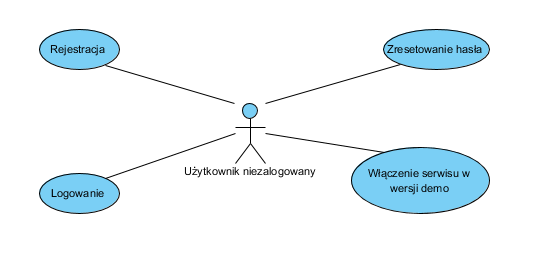
\includegraphics[scale=0.9]{assets/uml1.png}
		\caption[]{Diagram UML aktora niezalogowanego}
		\label{fig:niezalakt}
	\end{figure} 
	\paragraph*{} Zgodnie z rysunkiem \ref{fig:niezalakt} oraz wymaganiami funkcjonalnymi, użytkownik niezalogowany ma możliwość rejestracji, logowania, zresetowania hasła lub włączenia serwisu w wersji demo.
	\begin{figure}[H]
		\hspace*{-4cm} 
		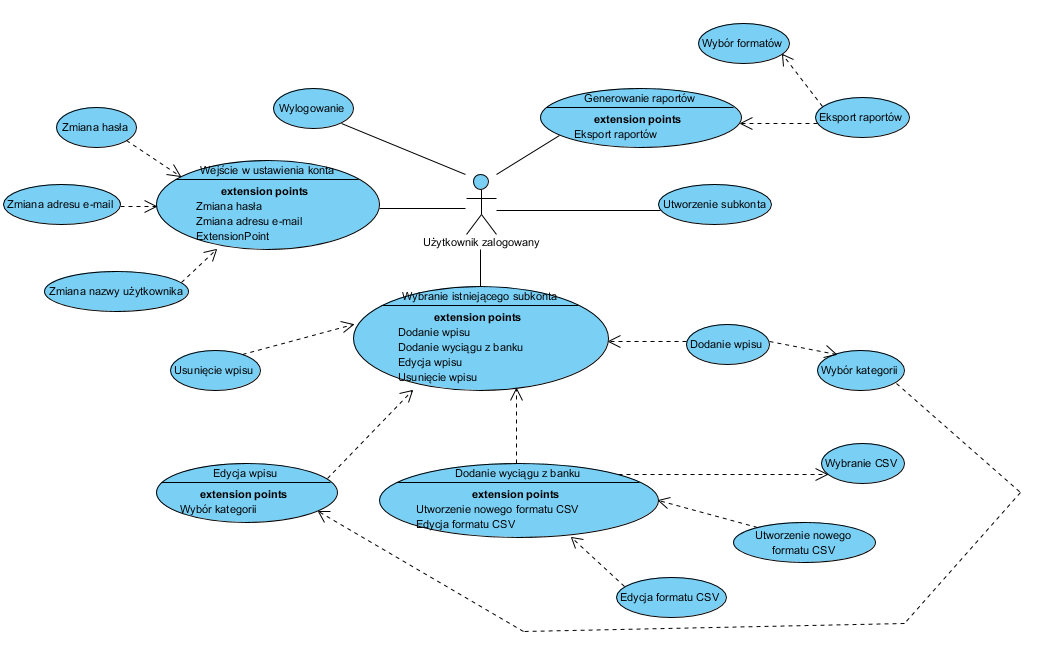
\includegraphics[scale=0.75]{assets/uml2.png}
		\caption[]{Diagram UML aktora zalogowanego}
		\label{fig:zalakt}
	\end{figure} 
	\paragraph*{} Zgodnie z rysunkiem \ref{fig:zalakt} oraz wymaganiami funkcjonalnymi, użytkownik zalogowany ma możliwość wylogowania; utworzenia subkonta; generowania raportów a w nim możliwość eksportu raportu oraz wybór formatu; wejścia w ustawienia konta, a w nim, zmianę hasła, zmianę adresu e-mail, zmianę nazwy użytkownika; wybranie istniejącego subkonta, a w nim, dodanie wpisu wraz z wyborem kategorii, dodanie wyciągu z banku wraz z edycją formatu CSV, utworzeniem nowego formatu CSV, czy wybraniem CSV, edycji wpisu oraz usunięcia wpisu.
	\subsection{Diagramy UML sekwencji}
	\paragraph*{} W tym paragrafie zostały przedstawione na rysunkach oraz opisane diagramy UML sekwencji dla użytkownika zalogowanego oraz użytkownika niezalogowanego. Są to diagramy sekwencji rejestracji użytkownika niezalogowanego, logowania użytkownika niezalogowanego, tworzenia subkonta przez użytkownika zalogowanego, dodawania wpisu przez użytkownika zalogowanego, dodawania wyciągu z banku użytkownika zalogowanego, modyfikacji oraz usuwania wpisów przez użytkownika zalogowanego oraz generowania raportów przez użytkownika zalogowanego.
	\begin{figure}[H]
		\hspace*{-2.5cm} 
		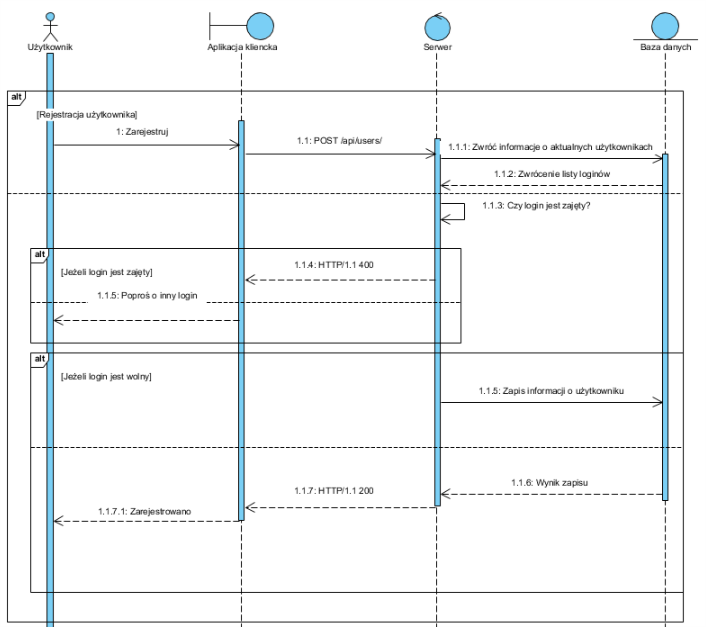
\includegraphics[scale=0.9]{assets/sq1.png}
		\caption[]{Diagram UML sekwencji rejestracji}
		\label{fig:umlreje}
	\end{figure} 
	\begin{figure}[H]
		\hspace*{-2.5cm} 
		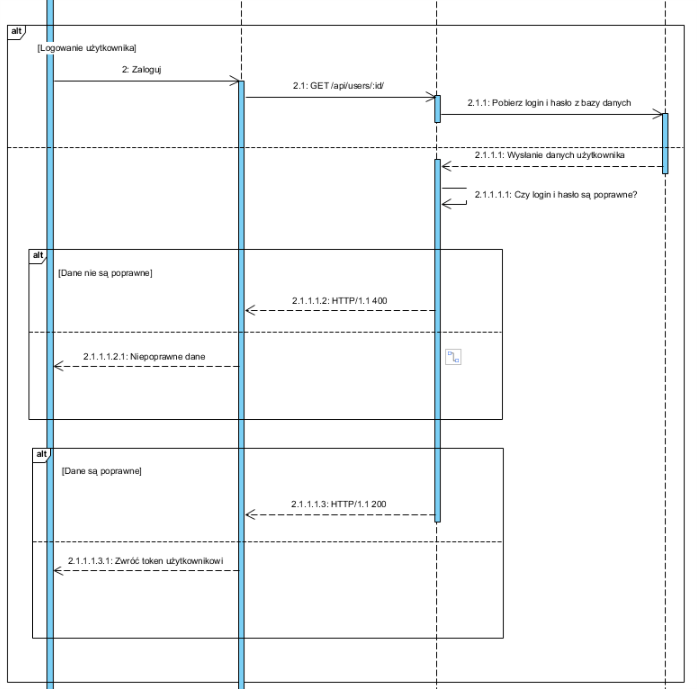
\includegraphics[scale=0.9]{assets/sq2.png}
		\caption[]{Diagram UML sekwencji logowania}
		\label{fig:umllog}
	\end{figure} 
	\begin{figure}[h]
		\vspace{-3.5cm}
		\hspace*{-2.5cm} 
		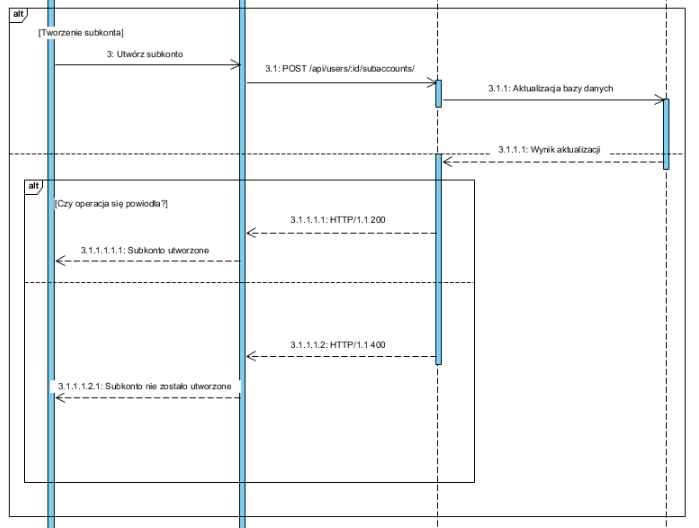
\includegraphics[scale=0.9]{assets/sq3.png}
		\caption[]{Diagram UML sekwencji tworzenia subkonta}
		\label{fig:umlsub}
	\end{figure} 
	\begin{figure}[H]
		
		\hspace*{-1.5cm} 
		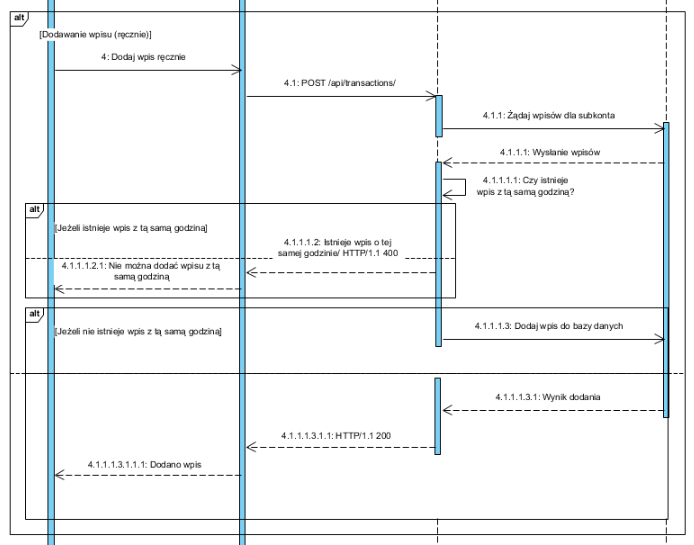
\includegraphics[scale=0.8]{assets/sq4.png}
		\caption[]{Diagram UML sekwencji dodawania wpisu}
		\label{fig:umlwpr}
	\end{figure} 
	\begin{figure}[H]
		
		\hspace*{-1.5cm} 
		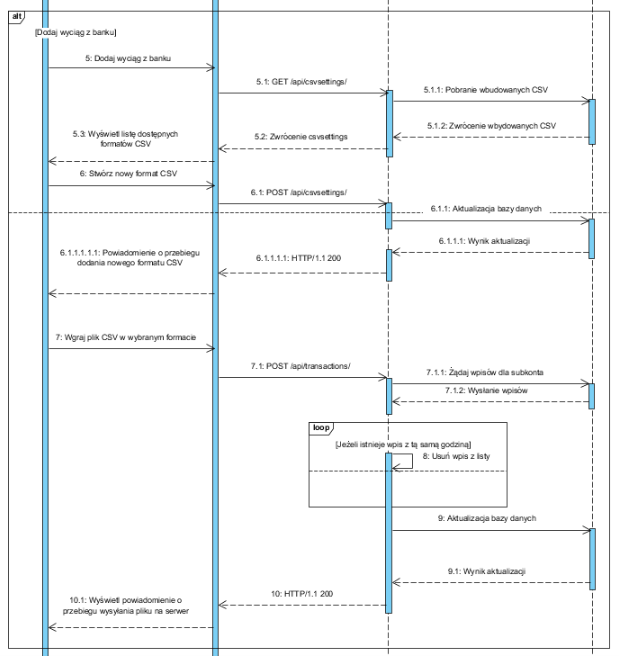
\includegraphics[scale=0.9]{assets/sq5.png}
		\caption[]{Diagram UML sekwencji dodawania wyciągu z banku}
		\label{fig:umlwpb}
	\end{figure}
	\begin{figure}[H]
		\hspace*{-1.5cm} 
		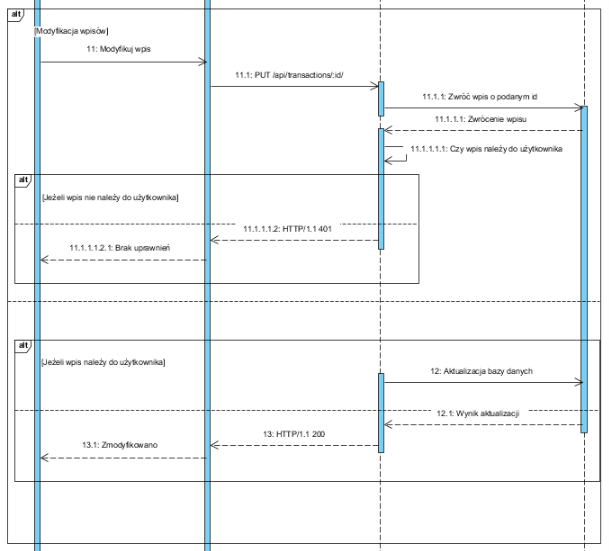
\includegraphics[scale=0.9]{assets/sq6.png}
		\caption[]{Diagram UML sekwecji modyfikacji wpisów}
		\label{fig:umlmod}
	\end{figure}  
	\begin{figure}[H]
		
		\hspace*{-1.5cm} 
		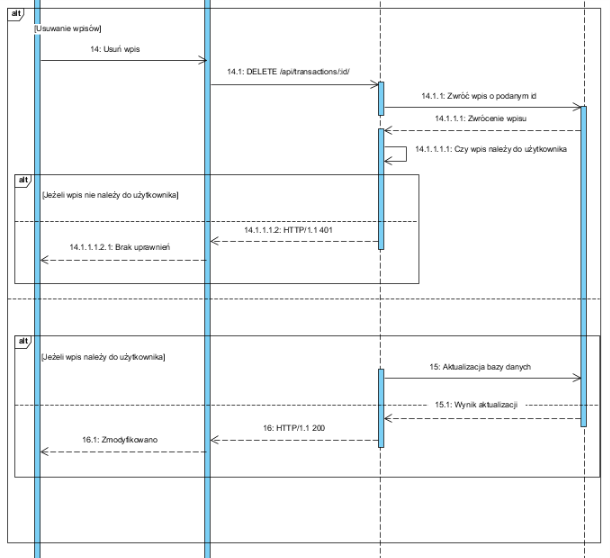
\includegraphics[scale=0.9]{assets/sq7.png}
		\caption[]{Diagram UML sekwencji usuwania wpisów}
		\label{fig:umlusu}
	\end{figure} 
	\begin{figure}[H]
		
		\hspace*{-1.5cm} 
		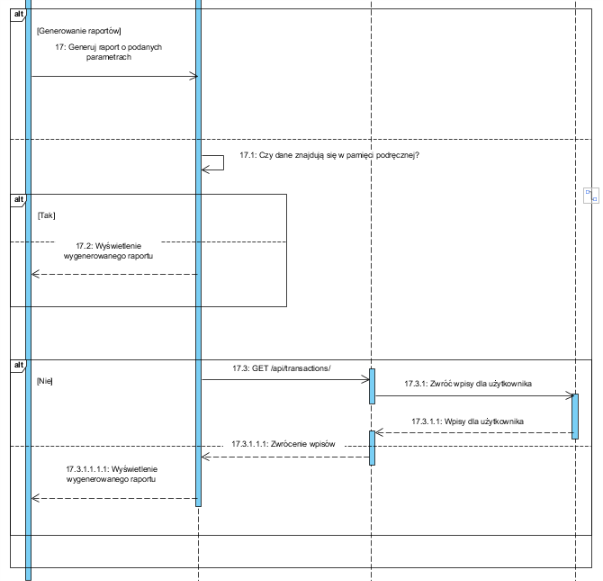
\includegraphics[scale=0.9]{assets/sq8.png}
		\caption[]{Diagram UML sekwencji generowania raportów}
		\label{fig:umlrap}
	\end{figure} 
	
	\section{Projekt interfejsu graficznego}
	\paragraph*{} W tym rozdziale został przedstawiony projekt interfejsu graficznego aplikacji klienckiej.
	
	\begin{figure}[H]
		\vspace*{-2cm}
		\hspace*{-2cm}
		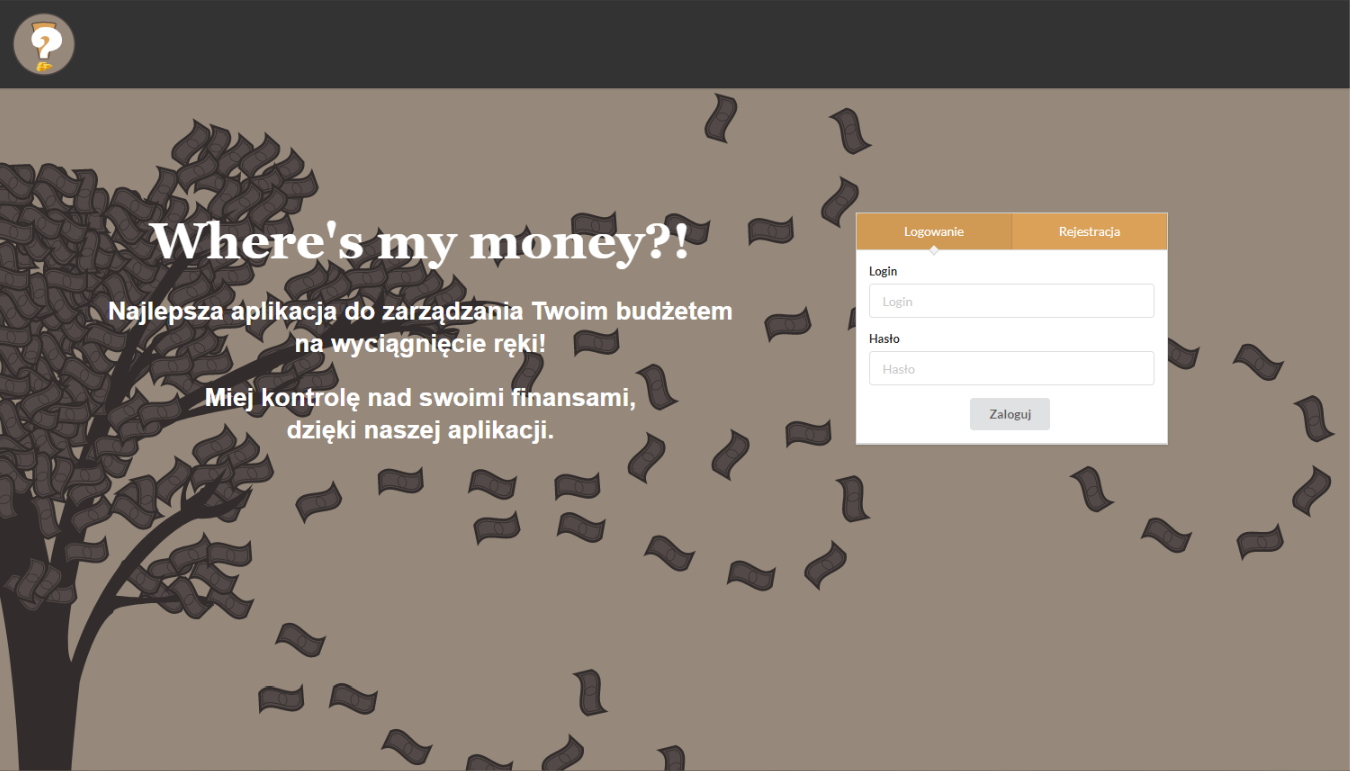
\includegraphics[scale=0.45]{assets/mc1.png}
		\caption[]{Interfejs ekranu logowania}
		\label{fig:logowanie}
	\end{figure} 
	\begin{figure}[H]
		\hspace*{-2cm}
		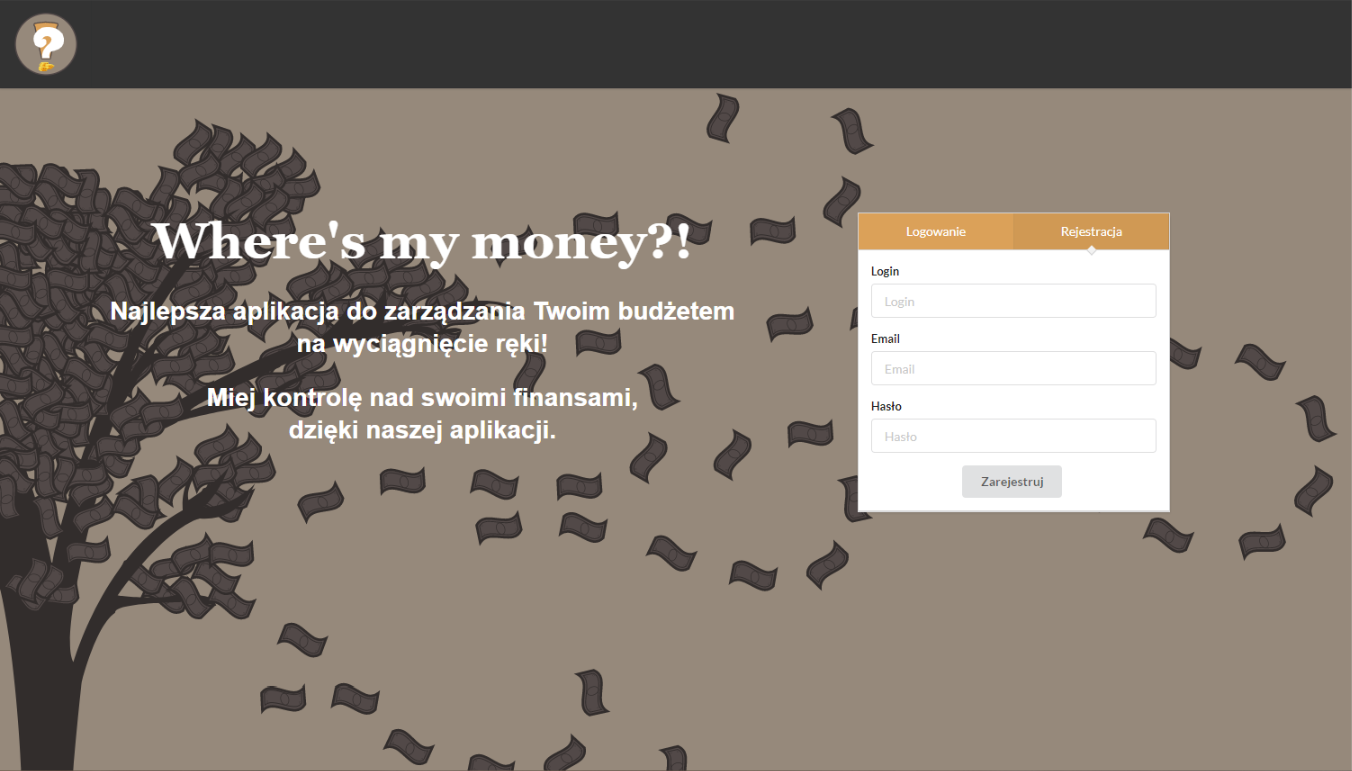
\includegraphics[scale=0.45]{assets/mc2.png}
		\caption[]{Interfejs ekranu rejestracji}
		\label{fig:rejestracja}
	\end{figure} 
\end{document}
